\documentclass{standalone}
\usepackage{tikz}
\usetikzlibrary{calc}

\pgfmathsetseed{1}
\pgfmathdeclarerandomlist{spin}{{$+$}{$-$}}
\pgfmathdeclarerandomlist{update_types}{{l}{r}{$\oplus$}{$\ominus$}}

\begin{document}
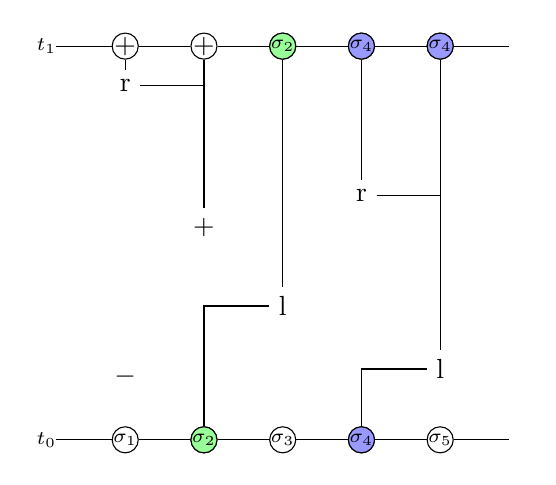
\begin{tikzpicture}

\def \n {5}
\def \height {5}

\definecolor{c_node_highlight}{RGB}{255,211,170}
% paletton.com
% Monochromatic with added complemntary
% base: 255E69

% Top and bottom nodes
\foreach \s in {1,...,\n} {
  \node (bottom\s) at (\s, 0) [circle, draw] {};
  \node (top\s) at (\s, \height) [circle, draw] {};
}

% Join nodes together
\foreach \s in {2, ..., \n} {
	\pgfmathparse{\s - 1}
	\draw (bottom\pgfmathresult) -- (bottom\s);
	\draw (top\pgfmathresult) -- (top\s);
}

%Nodes on edges
\node (bottomleft) at (0, 0){};
\node (bottomright) at (\n + 1, 0){};
\node (topleft) at (0, \height){};
\node (topright) at (\n + 1, \height){};
\draw (bottomleft) -- (bottom1);
\draw (bottomright) -- (bottom\n);
\draw (topleft) -- (top1);
\draw (topright) -- (top\n);



% Random updates (MAKE THIS DETERMINISTIC)
% \foreach \s in {1, ..., \n} {
% 	\pgfmathrandominteger{\m}{1}{3}
% 	\foreach \i in {1, ..., \m} {
% 		\pgfmathrandomitem{\updatetype}{update_types}
% 		\node at (\s, rnd * \height) [] {\updatetype};
% 	}
% }


% Important Updates
\node (update01) at (1,4.5) [] {r};
\node (update02) at (4, 3.1) [] {r};
\node (update03) at (2, 2.7) [] {$+$};
\node (update04) at (3, 1.7) [] {l};
\node (update05) at (5,0.9) [] {l};


% Percolation
\draw (top1) -- (update01) -- ($(update01) + (1,0)$);
\draw (top2) -- (update03);

\draw (top3) -- (update04);
\draw (update04) -- ($(update04) + (-1,0)$) -- (bottom2);

\draw (top4) -- (update02) -- ($(update02) + (1,0)$);
\draw (top5) -- (update05) -- ($(update05) + (-1,0)$) -- (bottom4);

% Unimportant Updates
\node at (1, 0.8) [] {$-$};


% Color matching final and inital spins
\node at (2, 0) [circle, draw, fill = green!40!white] {};
\node at (3, \height) [circle, draw, fill = green!40!white] {};

\node at (4, 0) [circle, draw, fill = blue!40!white] {};
\node at (4, \height) [circle, draw, fill = blue!40!white] {};
\node at (5, \height) [circle, draw, fill = blue!40!white] {};

% Final spins
\node at (1,\height) [] {$+$};
\node at (2,\height) [] {$+$};
\node at (3,\height) [] {\scriptsize $\sigma_2$};
\node at (4,\height) [] {\scriptsize $\sigma_4$};
\node at (5,\height) [] {\scriptsize $\sigma_4$};

% Initial spins
\node at (1, 0) [] {\scriptsize $\sigma_1$};
\node at (2, 0) [] {\scriptsize $\sigma_2$};
\node at (3, 0) [] {\scriptsize $\sigma_3$};
\node at (4, 0) [] {\scriptsize $\sigma_4$};
\node at (5, 0) [] {\scriptsize $\sigma_5$};

% Time labels
\node at (0,0) [] {\scriptsize$t_0$};
\node at (0,\height) [] {\scriptsize$t_1$};

\end{tikzpicture}
\end{document}